% Figure 1: Architecture diagram.
% Editable source: figures/fig1_architecture.drawio (draw.io).
% Publication rendering: figures/fig1_architecture.pdf (make_fig1.py renders the
% same diagram; a GUI export from draw.io is tracked as the final-export step).
% Mechanisms depicted are exactly those in the frozen implementation
% (FACTS.md F-DESIGN-HEAD / F-DESIGN-GATE / F-DESIGN-DETACH).
\begin{figure*}[!t]
\centering
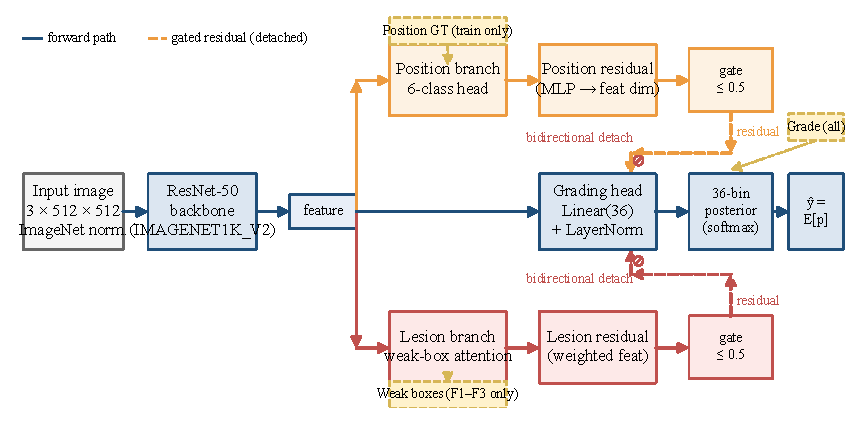
\includegraphics[width=0.98\textwidth]{figures/fig1_architecture.pdf}
\caption{Architecture of SynAP-Fib. The ResNet-50 backbone extracts features
from the normalized $3 \times 512 \times 512$ input. The grading head produces a
36-bin ordinal posterior via a linear output layer, from which the continuous
score is computed as the posterior expectation. The position branch (six-class
head) and lesion branch (spatial attention supervised by weak box unions)
inject their outputs into the grading pathway as residuals through learned
scalar gates (bounded above by $0.5$).
\textbf{Gradient flow is bidirectionally detached} at both injections:
auxiliary losses update their own branches only, and the grading loss does not
flow into the branch heads through the injection. Position ground truth is used
only during training; at inference the grading pathway reads the predicted
position posterior, requiring no anatomical metadata.}
\label{fig:architecture}
\end{figure*}
